\section*{Đề thi thử cụm Hà nội 1 25-26 Lần 1}
\caulc
\begin{ex}%[1D2H2-6]
	Cho một cấp số cộng có số hạng đầu là $u_1=3$, công sai $d=2$. Tổng $S_n$ của $n$ ($n\geq 1$) số hạng đầu tiên của cấp số cộng là
	\choice
	{\True $S_n=n^2+2n$}
	{$S_n=n^2+n$}
	{$S_n=\dfrac{2n^2+n}{2}$}
	{$S_n=\dfrac{3n^2+n}{2}$}
	\loigiai{
		Cấp số cộng có $u_1=3$, $d=2$.\\
		Ta có 
		\begin{align*}
			S_n&=\dfrac{n}{2}\left[2u_1+(n-1)d\right]\\
			&=\dfrac{n}{2}[2\cdot 3+(n-1)\cdot 2]\\
			&=\dfrac{n}{2}(6+2n-2)\\
			&=\dfrac{n}{2}(2n+4)\\
			&=n^2+2n.
		\end{align*}
	}
\end{ex}
\begin{ex}%[2D4N1-2]
	Khẳng định nào sau đây đúng?
	\choice
	{$\displaystyle\int \mathrm{e}\mathrm{\,d}x=\dfrac{\mathrm{e}^2}{2}+C$}
	{$\displaystyle\int \mathrm{e}\mathrm{\,d}x=\mathrm{e}^x+C$}
	{$\displaystyle\int \mathrm{e}\mathrm{\,d}x=\mathrm{e}+C$}
	{\True $\displaystyle\int \mathrm{e}\mathrm{\,d}x=\mathrm{e}x+C$}
	\loigiai{
		Vì $\mathrm{e}$ là hằng số nên $\displaystyle\int \mathrm{e}\mathrm{\,d}x=\mathrm{e}x+C$.
	}
\end{ex}
\begin{ex}%[2D1N4-1]
	Tiệm cận đứng của đồ thị hàm số $y=\dfrac{2x-1}{x+3}$ là
	\choice
	{\True $x=-3$}
	{$y=2$}
	{$y=-2$}
	{$x=3$}
	\loigiai{
		Ta có $\lim\limits_{x\to -3^-}\dfrac{2x-1}{x+3}=-\infty$.\\
		Vậy $x=-3$ là tiệm cận đứng của đồ thị hàm số.
	}
\end{ex}
\begin{ex}%[2D3H2-2]
	Bạn Anh thống kê lại chiều cao (đơn vị: cm) của các bạn học sinh nữ lớp $12$C ở bảng sau
	\begin{center}
		\begin{tabular}{|c|c|c|c|c|c|c|}
			\hline
			Chiều cao (cm) & $[155;160)$ & $[160;165)$ & $[165;170)$ & $[170;175)$ & $[175;180)$ & $[180;185)$ \\
			\hline
			Lớp $12$C & $2$ & $7$ & $12$ & $3$ & $2$ & $1$\\
			\hline
		\end{tabular}
	\end{center}
	Độ lệch chuẩn về chiều cao của mẫu số liệu (làm tròn đến hàng phần trăm) là
	\choice
	{$5{,}96$}
	{$6{,}95$}
	{\True $5{,}69$}
	{$6{,}59$}
	\loigiai{
		Lấy giá trị đại diện của các lớp là
		\begin{center}
			\begin{tabular}{|c|c|c|c|c|c|c|}
				\hline
				\multicolumn{1}{|c|}{Khoảng} & $[155;160)$ & $[160;165)$ & $[165;170)$ & $[170;175)$ & $[175;180)$ & $[180;185)$ \\
				\hline
				Giá trị đại diện & $157{,}5$ & $162{,}5$ & $167{,}5$ & $172{,}5$ & $177{,}5$ & $182{,}5$ \\
				\hline
				Tần số & $2$ & $7$ & $12$ & $3$ & $2$ & $1$ \\
				\hline
			\end{tabular}
		\end{center}
		Tổng số học sinh $n=2+7+12+3+2+1=27$.\\
		Số trung bình $\overline{x}=\dfrac{157{,}5\cdot 2+162{,}5\cdot 7+167{,}5\cdot 12+172{,}5\cdot 3+177{,}5\cdot 2+182{,}5\cdot 1}{27}\approx 167{,}31$.\\
		Độ lệch chuẩn $s=\sqrt{\dfrac{1}{27}\sum n_i\left(x_i-\overline{x}\right)^2}\approx 5{,}69$.
	}
\end{ex}
\begin{ex}%[2D4H3-3]
	Gọi $D$ là hình phẳng giới hạn bởi đồ thị hàm số $y=x^4$, trục hoành và hai đường thẳng $x=0$, $x=1$. Quay $D$ quanh trục $Ox$ ta được khối tròn xoay có thể tích bằng
	\choice
	{$\dfrac{\pi}{9}$}
	{$\dfrac{\pi}{5}$}
	{\True $\dfrac{1}{9}$}
	{$\dfrac{1}{5}$}
	\loigiai{		
		Thể tích khối tròn xoay là $V=\pi \displaystyle\int\limits_0^1\left(x^4\right)^2\mathrm{\,d}x=\pi \displaystyle\int\limits_0^1x^8\mathrm{\,d}x=\dfrac{\pi}{9}$.
	}
\end{ex}
\begin{ex}%[2H5H2-2]
	Trong không gian $Oxyz$, cho đường thẳng $(d)\colon\dfrac{x-1}{3}=\dfrac{2y+3}{2}=\dfrac{z-1}{2}$. Vectơ nào trong các vectơ có tọa độ sau đây là vectơ chỉ phương của đường thẳng $(d)$?
	\choice
	{$(3;2;-2)$}
	{\True$(3;1;2)$}
	{$(-3;-2;2)$}
	{$(3; 2;2)$}
	\loigiai{
		Đường thẳng $(d)$ được viết lại $\dfrac{x-1}{3}=\dfrac{y+\dfrac{3}{2}}{1}=\dfrac{z-1}{2}$.\\
		Vậy một vectơ chỉ phương của đường thẳng là $\overrightarrow{u}=(3;1;2)$.
	}
\end{ex}
\begin{ex}%[2H5H1-3]
	Trong không gian $Oxyz$, phương trình mặt phẳng đi qua ba điểm $A(1;0;0)$, $B(0;2;0)$, $C(0;0;-1)$ là
	\choice
	{$2x+y+z-2=0$}
	{$x-y-z+1=0$}
	{\True$2x+y-2z-2=0$}
	{$x+y+z-1=0$}
	\loigiai{
		Phương trình mặt phẳng $(ABC)$: 
		$\dfrac{x}{1}+\dfrac{y}{2}+\dfrac{z}{-1}=1\Leftrightarrow 2x+y-2z-2=0$.
	}
\end{ex}
\begin{ex}%[1D6H4-5]
	Số nghiệm nguyên của bất phương trình $\log _{\tfrac{1}{2}}(2x-1)\leq \log _{\tfrac{1}{2}}(-x+5)$ là
	\choice
	{\True $3$}
	{$2$}
	{$4$}
	{$1$}
	\loigiai{
		Ta có 
		\begin{align*}
			&\log _{\tfrac{1}{2}}(2x-1)\leq \log _{\tfrac{1}{2}}(-x+5)\\
			\Leftrightarrow&\heva{&2x-1\geq-x+5\\&-x+5>0}\\
			\Leftrightarrow&\heva{&x\geq2\\&x<5}\\
			\Leftrightarrow&2\leq x<5.
		\end{align*}
		Do $x$ là số nguyên, suy ra $x\in\{2;3;4\}$.\\
		Vậy phương trình đã cho có $3$ nghiệm nguyên.
	}
\end{ex}
\begin{ex}%[2H2H1-2]
	Cho hình lăng trụ tam giác $ABC.A'B'C'$. Vectơ $\overrightarrow{AA'}-\overrightarrow{AB}+\overrightarrow{AC}$ bằng vectơ nào sau đây?
	\choice
	{$\overrightarrow{B'C}$}
	{$\overrightarrow{C'B}$}
	{\True$\overrightarrow{BC'}$}
	{$\overrightarrow{B'C'}$}
	\loigiai{
		\begin{center}
		\begin{tikzpicture}[scale=1, font=\footnotesize, line join=round, line cap=round, >=stealth]
			\path 
			(0,0) coordinate (C)
			(4,0) coordinate (B)
			(1,-1) coordinate (A)
			(2,2) coordinate (A')
			($(A')+(B)-(A)$) coordinate (B')
			($(A')+(C)-(A)$) coordinate (C')
			;
			\draw (A')--(B')--(C')--cycle  (C')--(C)--(A)--(B)--(B') (A)--(A');
			\draw [dashed] (C)--(B);
			\foreach \d/\g in {A/-90, B/-45,C/180,A'/90,B'/45,C'/135}
			\fill (\d) circle(1pt) + (\g:.3) node{$\d$};
		\end{tikzpicture}
		\end{center}	
		Ta có 
		\begin{align*}
			\overrightarrow{AA'}-\overrightarrow{AB}+\overrightarrow{AC}&=\overrightarrow{AA'}+\overrightarrow{AC}-\overrightarrow{AB}\\
			&=\overrightarrow{AA'}+\overrightarrow{BC}\\
			&=\overrightarrow{CC'}+\overrightarrow{BC}\\
			&=\overrightarrow{BC'}.
		\end{align*}
	}
\end{ex}
\begin{ex}%[2H5H3-2]
	Trong không gian $Oxyz$ cho mặt cầu $(C)\colon x^2+y^2+z^2+2y-3=0$. Tọa độ tâm $I$ và bán kính $R$ của mặt cầu là
	\choice
	{\True$I(0;-1;0)$, $R=2$}
	{$I(0;-1;0)$, $R=4$}
	{$I(0;1;0)$, $R=2$}
	{$I(0;1;0)$, $R=4$}
	\loigiai{
		Từ phương trình $(C)\colon x^2+y^2+z^2+2y-3=0$, suy ra $a=0$, $b=-1$, $c=0$, $d=-3$.\\
		Suy ra mặt cầu có tâm $I(0;-1;0)$, bán kính $R=\sqrt{0^2+(-2)^2+0^2-(-3)}=2$.
	}
\end{ex}
\begin{ex}%[2D1N2-2]
	Cho hàm số $f(x)$ có bảng biến thiên như sau
	\begin{center}
		
\begin{tikzpicture}
			\tkzTabInit[nocadre=true,lgt=1.2,espcl=3, deltacl=0.5]
			{$x$/0.7,$f'(x)$/0.7,$f(x)$/2}
			{$-\infty$,$-1$,$2$,$+\infty$}
			\tkzTabLine{,-,$0$,+,$0$,-,}
			\tkzTabVar{+/$+\infty$,-/$-2$,+/$3$,-/$-\infty$}
		\end{tikzpicture}
	\end{center}
	Giá trị cực tiểu của hàm số là
	\choice
	{\True$-2$}
	{$2$}
	{$3$}
	{$-1$}
	\loigiai{
		Từ bảng biến thiên, suy ra giá trị cực tiểu của hàm số bằng $-2$.
	}
\end{ex}
\begin{ex}%[1H8N7-1]
	Cho một khối lăng trụ có diện tích đáy bằng $a^2\sqrt{3}$ và có thể tích bằng $3a^3$. Chiều cao của khối lăng trụ là
	\choice
	{$a$}
	{$\dfrac{a}{\sqrt{3}}$}
	{$3a\sqrt{3}$}
	{\True$a\sqrt{3}$}
	\loigiai{
		Thể tích khối lăng trụ là $V=S_{\text{đáy }}\cdot h$.\\
		Theo đề ra ta có $S_{\text{đáy }}=a^2\sqrt{3}$, $V=3a^3$.\\
		Suy ra $h=\dfrac{V}{S_{\text{đáy }}}=\dfrac{3a^3}{a^2\sqrt{3}}=\dfrac{3a}{\sqrt{3}}=a\sqrt{3}$.
	}
\end{ex}
\cauds
\begin{ex}%[2H2V2-4]
	Một bể cá cảnh có mô hình bên trong là hình hộp chữ nhật $ABCD.A'B'C'D'$ với $AD=4$\,dm, $AB=8$\,dm, $AA'=4$\,dm. Trong quá trình thay nước cho bể cá người ta rút bớt nước trong bể, phần nước còn lại khi nghiêng bể thì người ta thấy bề mặt thoáng của nước trong bể là tứ giác $CBHK$, trong đó $H$, $K$ lần lượt là trung điểm của $AA'$, $DD'$ (tham khảo hình vẽ $1$). Sau khi bể nước được đặt trở lại vị trí thăng bằng thì mặt thoáng của nước trong bể là tứ giác $MNPQ$, toàn bộ khối được đặt trong hệ trục tọa độ $Oxyz$ như hình vẽ $2$; gốc $O$ trùng với $A$, tia $Ox$ trùng với tia $AD$, tia $Oy$ trùng với tia $AB$, tia $Oz$ trùng với tia $AA'$.
	\begin{center}
		\begin{tikzpicture}[scale=1, font=\footnotesize, line join=round, line cap=round, >=stealth]
			\path 
			(0,0) coordinate (K)
			(5,0) coordinate (C)
			(6,.6) coordinate (B)
			($(K)+(B)-(C)$)coordinate (H)
			($(-150:2.5)+(2.5,0)$) coordinate (D)
			($(D)!2!(K)$) coordinate (D')
			($(D)+(B)-(C)$)coordinate (A)
			($(D')+(A)-(D)$)coordinate (A')
			($(B)+(A')-(A)$)coordinate (B')
			($(B')+(C)-(B)$)coordinate (C')
			;
			\fill[green!50] (D)--(K)--(C)--cycle;
			\fill[green!20] (K)--(H)--(B)--(C)--cycle;
			\draw (C)--(D)--(D')--(C')--(C) (D)--(D') (K)--(C)--(B)--(B')--(C') (D')--(A')--(B') ;
			\draw[dashed] (K)--(H)--(B) (D)--(A)--(B) (A)--(A');
			\foreach \d/\g in {D/-135,C/-45,B/-45,A/160,K/180,H/160,D'/160,A'/120,B'/90,C'/160}
			\fill (\d) circle(1pt) + (\g:.25) node{$\d$};
			\fill (2.5,-2)	node{Hình vẽ 1};
		\end{tikzpicture}
		\quad\quad
		\begin{tikzpicture}[scale=1, font=\footnotesize, line join=round, line cap=round, >=stealth]
			\path 
			(0,0) coordinate (A)
			(5,0) coordinate (B)
			(-1,-.4) coordinate (D)
			($(B)+(D)-(A)$)coordinate (C)
			($(D)+(0,2.5)$) coordinate (D')
			($(D')+(A)-(D)$)coordinate (A')
			($(B)+(A')-(A)$)coordinate (B')
			($(B')+(C)-(B)$)coordinate (C')
			($(B)!.25!(B')$)coordinate (P)
			($(A)!.25!(A')$)coordinate (M)
			($(C)!.25!(C')$)coordinate (N)
			($(D)!.25!(D')$)coordinate (Q)
			($(A)!1.25!(B)$)coordinate (y)
			($(A)!1.5!(D)$)coordinate (x)
			($(A)!1.35!(A')$)coordinate (z)
			;
			\fill[green!20] (Q)--(M)--(P)--(N)--cycle;
			\fill[green!50] (N)--(Q)--(D)--(C)--cycle;
			\fill[green!50] (N)--(P)--(B)--(C)--cycle;
			\draw [->](B)--(y);
			\draw [->](D)--(x);
			\draw [->](A')--(z);
			\draw (D)--(C)--(B) (Q)--(N)--(P) (A')--(B')--(C')--(D')--cycle (D)--(D') (C)--(C') (B)--(B');
			\draw[dashed] (D)--(A)--(B) (A)--(A') (Q)--(M)--(P);
			\foreach \d/\g in {D/-65,C/-45,B/-65,A/-45,D'/135,A'/45,B'/45,C'/120,Q/180,N/120,P/-45,M/135}
			\fill (\d) circle(1pt) + (\g:.25) node{$\d$};
			\foreach \d/\g in {x/-90,y/-90,z/180}
			\fill (\d) + (\g:.25) node{$\d$};
			\fill (2.5,-2)	node{Hình vẽ 2};	
		\end{tikzpicture}	
	\end{center}
	\choiceTF
	{\True Bể cá cảnh có thể chứa được tối đa $128$ lít nước}
	{Thể tích nước còn lại trong bể không vượt quá $30$ lít}
	{Người ta muốn đặt một bóng đèn trang trí tại trọng tâm $G$ của tam giác $APQ$. Tọa độ $G\left(\dfrac{16}{3};\dfrac{4}{3};\dfrac{4}{3}\right)$}
	{\True Người ta làm một dây sục khí cho bể cá là một cung tròn có điểm bắt đầu tại $A'$ đi qua điểm $E(2;1;1)$ và kết thúc tại điểm $F(4;2;0)$. Độ dài của dây sục khí theo đơn vị đềximét thuộc khoảng $(6{,}2;6{,}3)$}
	\loigiai{
		\begin{itemchoice}
			\itemch	Thể tích của bể là $V=4\cdot 8\cdot 4=128\,(\text{dm}^3)=128$ lít.
			\itemch Khi nghiêng bể, mặt thoáng nước là tứ giác $CBHK$, trong đó $H$, $K$ là trung điểm của $AA'$, $DD'$. Khi đó phần nước còn lại là một lăng trụ tam giác có chiều cao $AD=4$\,dm, đáy là tam giác có hai cạnh góc vuông là $8$\,dm và $2$\,dm.\\
			Thể tích nước còn lại là $V=4\cdot \dfrac{1}{2}\cdot 8\cdot 2=32\,(\text{dm}^3)=32$ (lít).
			\itemch Sau khi đặt bể trở lại vị trí thăng bằng, ta có
			$$V=DA\cdot AD\cdot AB\Leftrightarrow 32=DQ\cdot 4\cdot 8\Rightarrow DQ=1.$$			
			Do đó chiều cao mực nước là $1$\,(dm).\\
			Suy ra $P(0;8;1)$, $Q(4;0;1)$.\\
			Toạ độ trọng tâm của tam giác $APQ$ là $G\left(\dfrac{4}{3};\dfrac{8}{3};\dfrac{2}{3}\right)$.
			\itemch 
			\begin{center}
				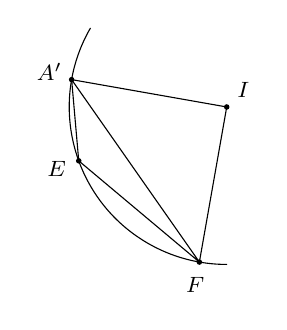
\begin{tikzpicture}[scale=1, font=\footnotesize, line join=round, line cap=round, >=stealth]
					\path 
					(0,0) coordinate (I)
					(170:2) coordinate (A')
					(200:2) coordinate (E)
					(260:2) coordinate (F)
					;
					\draw (I)--(A')--(E)--(F)--cycle (A')--(F);
					\draw (150:2) arc (150:270:2);
					\foreach \d/\g in {A'/160, I/45,E/200,F/260}
					\fill (\d) circle(1pt) + (\g:.3) node{$\d$};
				\end{tikzpicture}
			\end{center}
			Ta có $A'(0;0;4)$, $E(2;1;1)$, $F(4;2;0)$.\\ 
			Suy ra $A'E=\sqrt{14}$, $EF=\sqrt{6}$, $A'F=6$.\\
			Gọi $I$ là tâm đường tròn ngoại tiếp tam giác $A'EF$.\\
			Diện tích tam giác $A'EF$ theo công thức Hê-rông là $S=\sqrt{5}$.\\
			Bán kính đường tròn ngoại tiếp tam giác $A'EF$ là
			$R=\dfrac{A'E\cdot EF\cdot A'F}{4S}=\dfrac{3\sqrt{105}}{5}\approx 6{,}148$.\\		
			Ta có $\cos \widehat{A'IF}=\dfrac{IA'^2+ID^2-A'F^2}{2\cdot IA\cdot IF}=\dfrac{R^2+R^2-A'F^2}{2\cdot R\cdot R}\approx 0{,}5237$.\\
			Suy ra $\widehat{A'IF}\approx1{,}0195$ (rad).\\			
			Độ dài cung tròn từ $A'$ qua $E$ đến $F$ gần bằng $1{,}0195\cdot 6{,}148\approx 6{,}27$\,dm, thuộc khoảng $(6{,}2;6{,}3)$.
		\end{itemchoice}
	}
\end{ex}
\begin{ex}%[2D4V1-2]
	\immini{
	Cho hàm số $f(x)=\dfrac{ax+b}{cx+d}$ với $a$, $b$, $c$, $d\in \mathbb{R}$ có đồ thị hàm số $f'(x)$ nhận đường thẳng $x=1$ làm tiệm cận đứng như hình vẽ bên. Biết rằng giá trị nhỏ nhất của hàm số $f(x)$ trên $[2;4]$ bằng $6$.
	\choiceTF
{Hàm số $f(x)$ đồng biến trên khoảng $(1;+\infty)$}
{Giá trị của $f(2)$ bằng $6$}
{\True Giá trị $\dfrac{a+b}{2c-d}$ bằng $1$}
{\True Có $4$ điểm điểm trên đồ thị hàm số $y=f(x)$ có tọa độ nguyên}
}{\begin{tikzpicture}[scale=0.7, font=\footnotesize, line join=round,
	line cap=round, >=stealth]
	\def \xmin{-2.5}
	\def \xmax{4}
	\def \ymin{-4}
	\def \ymax{2}
	\draw[->] (\xmin,0)--(\xmax,0) node[shift=(90:0.2)] {$x$};
	\draw[->] (0,\ymin)--(0,\ymax) node[shift=(-150:0.2)] {$y$};
	\fill (0,0) circle(1pt) node[shift=(-45:0.25)]{$O$}
	(1,0) circle(1pt) node[shift=(135:0.2)]{$1$}
	(0,-3) circle(1pt) node[shift=(180:0.27)]{$-3$};
	\clip (\xmin,\ymin) rectangle (\xmax,\ymax);
	\draw[smooth,samples=100,domain=\xmin:0.9] plot(\x,{ -3/((\x-1)^2) });
	\draw[smooth,samples=100,domain=1.1:\xmax] plot(\x,{ -3/((\x-1)^2) });
	\draw (1,\ymax)--(1,\ymin);
	\end{tikzpicture}}
	\loigiai{
		\begin{itemchoice}
			\itemch Ta có $f(x)=\dfrac{ax+b}{cx+d}$ nên $f'(x)=\dfrac{ad-bc}{(cx+d)^2}$.\\
			Từ đồ thị $f'(x)$, đường thẳng $x=1$ là tiệm cận đứng nên $cx+d=0$ tại $x=1$.\\
			Suy ra $d=-c$.\\
			Do đó $f'(x)$ có dạng $f'(x)=\dfrac{k}{(x-1)^2}$.\\
			Từ đồ thị thấy $f'(0)=-3$, nên $k=-3$.\\
			Suy ra $f'(x)=\dfrac{-3}{(x-1)^2}$.\\
			Vì $f'(x)<0$ trên $(1;+\infty)$ nên $f(x)$ nghịch biến trên $(1;+\infty)$.
			\itemch 
			Ta có $f(x)=\displaystyle\int f'(x)\mathrm{\,d}x =\displaystyle\int \dfrac{-3}{(x-1)^2}\mathrm{\,d}x =\dfrac{3}{x-1}+C$.\\
			Trên $[2;4]$, hàm số nghịch biến nên giá trị nhỏ nhất đạt tại $x=4$.\\
			Theo đề, $\min\limits_{[2;4]}f(x)=6$, suy ra $f(4)=6$.\\			
			Do đó $\dfrac{3}{4-1}+C=6\Rightarrow C=5$.\\
			Suy ra $f(x)=5+\dfrac{3}{x-1}=\dfrac{5x-2}{x-1}$.\\
			Vậy $f(2)=5+\dfrac{3}{1}=8$.
			\itemch Từ $f(x)=\dfrac{5x-2}{x-1}$, suy ra $a=5$, $b=-2$, $c=1$, $d=-1$.\\
			Khi đó $\dfrac{a+b}{2c-d}=\dfrac{5-2}{2\cdot 1-(-1)}=\dfrac{3}{3}=1$
			\itemch Để điểm trên đồ thị có tọa độ nguyên, cần $x$ nguyên và $y=5+\dfrac{3}{x-1}$ nguyên.\\
			Suy ra $x-1\in \text{Ư}(3)$, tức là $x-1\in\{-3;-1;1;3\}$, suy ra $x\in\{-2;0;2;4\}$.\\
			Vậy $4$ giá trị nguyên của $x$, nên có $4$ điểm có tọa độ nguyên.
		\end{itemchoice}
	}
\end{ex}
\begin{ex}%[2D4V2-6]
	Một hạt chuyển động thẳng trên trục $Ox$ và xuất phát tại $O$. Phương trình chuyển động của hạt là $x(t)=t-2\ln (t+1)$ (đơn vị: mét), trong đó $t$ là thời gian tính bằng giây. Hàm số $v(t)=x'(t)$ (đơn vị: mét/giây) biểu thị vận tốc chuyển động của hạt.
	\choiceTF
	{$v(t)=2-\dfrac{3}{t+1}$}
	{Vận tốc ban đầu của hạt là $2$ m/s}
	{\True Vận tốc tức thời tại thời điểm $t=1$ s là $0$ m/s}
	{\True Quãng đường hạt đi được trong $4$ giây đầu tiên (làm tròn kết quả đến hàng phần trăm) là $1,55$ m}
	\loigiai{	
		\begin{itemchoice}
			\itemch Vận tốc là $v(t)=x'(t)=1-\dfrac{2}{t+1}$.
			\itemch Vận tốc ban đầu là $v(0)=1-\dfrac{2}{1}=-1$ (m/s).
			\itemch Tại $t=1$, ta có $v(1)=1-\dfrac{2}{2}=0$ (m/s).
			\itemch Quãng đường hạt đi được trong $4$ giây đầu tiên là
			$$S=\displaystyle\int\limits_0^4 |v(t)|\mathrm{\,d}t=\displaystyle\int\limits_0^4\left|1-\dfrac{2}{t+1}\right|\mathrm{\,d}t\approx 1{,}55\, \text{(m)}.$$
		\end{itemchoice}
	}
\end{ex}
\begin{ex}%[2D6V2-3]
	Một sản phẩm do hai nhà máy $A$ và $B$ sản xuất. Tỉ lệ phế phẩm của nhà máy $A$ là $4\%$, của nhà máy $B$ là $1\%$. Trong một lô hàng có $120$ sản phẩm của nhà máy $A$; $80$ sản phẩm của nhà máy $B$. Lấy ngẫu nhiên một sản phẩm từ lô hàng.
	\choiceTF
	{\True Xác suất lấy được sản phẩm do nhà máy $A$ sản xuất là $0,6$}
	{\True Xác suất lấy được sản phẩm tốt biết rằng sản phẩm đó thuộc nhà máy $A$ bằng $0,96$}
	{Xác suất lấy được sản phẩm tốt là $0,964$}
	{Biết sản phẩm lấy ra là sản phẩm tốt. Xác suất sản phẩm đó do nhà máy $B$ sản xuất lớn hơn xác suất do nhà máy $A$ sản xuất}
	\loigiai{
		Gọi 
		\begin{itemize}
			\item $A$ là biến cố \lq\lq Lấy được sản phẩm nhà máy A\rq\rq.\\ 
			Suy ra $\overline{A}$ là biến cố \lq\lq Lấy được sản phẩm nhà máy B\rq\rq.			
			\item $B$ là biến cố \lq\lq Lấy được sản tốt\rq\rq.
		\end{itemize}		
		\begin{itemchoice}
			\itemch Tổng số sản phẩm là $120+80=200$.\\
			Suy ra $\mathrm{P}(A)=\dfrac{120}{200}=0{,}6$.
			\itemch Tỉ lệ phế phẩm của nhà máy $A$ là $4\%$, nên tỉ lệ sản phẩm tốt của nhà máy $A$ là $$1-0{,}04=0{,}96.$$
			\itemch 
			Ta có $\mathrm{P}(A)=0{,}6$, $\mathrm{P}\left(\overline{A}\right)=0{,}4$, $\mathrm{P}\left(B\mid\overline{A}\right)=1-0{,}01=0{,}99$, $\mathrm{P}(B\mid A)=1-0{,}04=0{,}96$.\\
			Xác suất lấy được sản phẩm tốt là
			$$\mathrm{P}(B)=\mathrm{P}(A)\cdot \mathrm{P}(B\mid A)+\mathrm{P}\left(\overline{A}\right)\cdot \mathrm{P}\left(B\mid \overline{A}\right)=0{,}6\cdot 0{,}96+0{,}4\cdot 0{,}99=0{,}972.$$
			\itemch 
			Ta có 
			\begin{itemize}
				\item $\mathrm{P}(A\mid B)=\dfrac{\mathrm{P}(A)\cdot \mathrm{P}(B\mid A)}{\mathrm{P}(B)}=\dfrac{0{,}6\cdot 0{,}96}{0{,}972}=\dfrac{0{,}576}{0{,}972}\approx 0{,}593$.
				\item $\mathrm{P}\left(\overline{A}\mid B\right)=\dfrac{\mathrm{P}(A)\cdot \mathrm{P}\left(\overline{A}\mid B\right)}{\mathrm{P}(B)}=\dfrac{0{,}4\cdot 0{,}99}{0{,}972}=\dfrac{0{,}396}{0{,}972}\approx 0{,}407$.
			\end{itemize}		
			Vì $0{,}407<0{,}593$, nên xác suất sản phẩm tốt đó do nhà máy $B$ sản xuất không lớn hơn xác suất do nhà máy $A$ sản xuất.
		\end{itemchoice}
	}
\end{ex}
\caukq
\begin{ex}%[2D4C3-2]
	\immini{
	Cho hình chữ nhật $ABCD$ tâm $O$, với $AB=6$, $BC=4$. Gọi $E$, $F$, $G$, $H$ lần lượt là trung điểm của $CD$, $AB$, $BC$, $AD$. Biết hai cung $GEH$, $GFH$ lần lượt là cung tròn đi qua $G$, $H$, $E$ và $G$, $F$, $H$. Tính diện tích phần hình được gạch sọc (làm tròn đến hàng phần chục).
}{\begin{tikzpicture}[scale=.75, font=\footnotesize, line join=round, line cap=round, >=stealth]
	\path 
	(0,0) coordinate (O)
	(3,0) coordinate (H)
	(-3,0) coordinate (G)
	(3,2) coordinate (D)
	(-3,2) coordinate (C)
	(-3,-2) coordinate (B)
	(3,-2) coordinate (A)
	(-3,2) coordinate (C)
	(0,2) coordinate (E)
	(0,-2) coordinate (F)
	;
	\begin{scope}
		\begin{scope}
			\clip (0,-1.25) circle(3.25);
			\begin{scope}
				\clip (0,1.25) circle(3.25);
				\draw[] (0,1.25) circle(3.25);
				\draw[pattern=north west lines] (0,-1.25) circle(3.25);	
			\end{scope}
		\end{scope}
		\fill[white,draw=black] (G)--(E)--(H)--(F)--cycle;
	\end{scope}
	\draw (A)--(B)--(C)--(D)--cycle (G)--(H) (E)--(F);
	\foreach \d/\g in {A/-45, D/45, C/135, B/-135, O/-45,H/0,G/180,E/90,F/-90}
	\fill (\d) circle(1pt) + (\g:.3) node{$\d$};
	\draw pic[draw,angle radius=2mm] {right angle = E--O--G};
\end{tikzpicture}
}
	\par
	\shortans{5,3}
	\loigiai{
		\begin{center}
			\begin{tikzpicture}[scale=.75, font=\footnotesize, line join=round, line cap=round, >=stealth]
				\path 
				(0,0) coordinate (O)
				(3,0) coordinate (H)
				(-3,0) coordinate (G)
				(3,2) coordinate (D)
				(-3,2) coordinate (C)
				(-3,-2) coordinate (B)
				(3,-2) coordinate (A)
				(-3,2) coordinate (C)
				(0,2) coordinate (E)
				(0,-2) coordinate (F)
				;
				\begin{scope}
					\begin{scope}
						\clip (0,-1.25) circle(3.25);
						\begin{scope}
							\clip (0,1.25) circle(3.25);
							\draw[] (0,1.25) circle(3.25);
							\draw[pattern=north west lines] (0,-1.25) circle(3.25);	
						\end{scope}
					\end{scope}
					\fill[white,draw=black] (G)--(E)--(H)--(F)--cycle;
				\end{scope}
				\draw (A)--(B)--(C)--(D)--cycle (G)--(H) (E)--(F);
				\foreach \d/\g in {A/-45, D/45, C/135, B/-135, O/-45,H/-45,G/-135,E/135,F/-45}
				\fill (\d) circle(1pt) + (\g:.3) node{$\d$};
				\draw pic[draw,angle radius=2mm] {right angle = E--O--G};
				\draw[->] (-4,0)--(4,0) node[above]{$x$};
				\draw[->] (0,-3)--(0,3) node[left]{$y$};
			\end{tikzpicture}
		\end{center}
		Đặt hệ trục tọa độ với tâm hình chữ nhật là $O(0;0)$.\\
		Suy ra $G(-3;0)$, $H(3;0)$, $E(0;2)$, $F(0;-2)$.\\
		Xét cung tròn $GEH$.\\
		Do tính đối xứng của hình, suy ra tâm $I$ của đường tròn đi qua ba điểm $G$, $H$, $E$ nằm trên trục $Oy$, suy ra $I(0;a)$.\\
		Ta có $IG=IE\Leftrightarrow IG^2=IE^2\Leftrightarrow 9+a^2=(2-a)^2\Leftrightarrow 9+a^2=4-4a+a^2\Leftrightarrow a=-\dfrac{5}{4}$.\\
		Suy ra $I\left(0;-\dfrac{5}{4}\right)$.\\
		Bán kính đường tròn là $R=IE=\sqrt{0+\left(2+\dfrac{5}{4}\right)^2}=\dfrac{13}{4}$.\\
		Phương trình đường tròn tâm $I$ bán kính $R$ là $x^2+\left(y+\dfrac{5}{4}\right)^2=\dfrac{169}{16}$.\\
		Suy ra phương trình nửa đừng tròn có chứa cung $HEG$ là $y=-\dfrac{5}{4}+\sqrt{\dfrac{169}{16}-x^2}$.\\
		Phương trình đừng thẳng $EH$ là $\dfrac{x}{3}+\dfrac{y}{2}=1\Rightarrow y=2-\dfrac{2x}{3}$.\\
		Diện tích hình phẳng giới hạn bởi cung cung tròn $EH$ và day cung $EH$ là
		$$S=\displaystyle\int\limits_0^3\left|-\dfrac{5}{4}+\sqrt{\dfrac{169}{16}-x^2}-\left(2-\dfrac{2x}{3}\right)\right|\mathrm{\,d}x-\dfrac{1}{2}\cdot 2\cdot 3\approx 1{,}336.$$
	Vậy tổng diện tích phần gạch sọc là $4\cdot 1{,}336\approx 5{,}3$.
	}
\end{ex}
\begin{ex}%[1D6H1-2]
	Giả sử cường độ ánh sáng $I$ dưới mặt nước biển giảm dần theo độ sâu theo công thức $I=I_0\cdot a^d$, trong đó $I_0$ là cường độ ánh sáng tại mặt nước biển, $a$ là một hằng số dương, $d$ là độ sâu tính từ mặt nước biển (đơn vị mét). Ở một vùng biển, cường độ ánh sáng tại độ sâu $1$ m bằng $95\%$ cường độ ánh sáng tại mặt nước biển. Tính tỷ lệ giữa cường độ ánh sáng tại độ sâu $20$ m so với cường độ ánh sáng tại độ sâu $10$ m ở vùng biển đó (làm tròn đến hàng phần chục).
	\par
	\shortans{0,6}
	\loigiai{
		Công thức cường độ ánh sáng là
		$$I=I_0\cdot a^d$$
		Tại độ sâu $1$ m, cường độ ánh sáng bằng $95\%$ cường độ ánh sáng tại mặt nước biển, ta có\\
		$$I_0\cdot a=0{,}95I_0\Rightarrow a=0{,}95$$
		Ta có
		$$\dfrac{I_{20}}{I_{10}}=\dfrac{I_0\cdot a^{20}}{I_0\cdot a^{10}}=a^{10}=0{,}95^{10}\approx 0{,}6$$
		Vậy $\dfrac{I_{20}}{I_{10}}\approx 0{,}6$.
	}
\end{ex}
\begin{ex}%[2D1V3-6]
	Gia đình anh Tuấn có mảnh đất, một phần giáp với đường (là một phần của đường thẳng), phần còn lại giáp với hồ nước là đường cong được mô hình hóa bởi một phần của đồ thị hàm số $f(x)=\dfrac{-x^2+5x-4}{x}$ như hình vẽ bên dưới, đơn vị trên mỗi trục tọa độ là $10$ mét. Trong mảnh đất anh Tuấn muốn rào một khu vực hình chữ nhật $ABCD$ với hai đỉnh $A$, $B$ nằm trên đồ thị hàm số $f(x)$ (phần giáp hồ) và cạnh $CD$ nằm trên trục hoành (phần giáp đường). Diện tích hình chữ nhật $ABCD$ đạt giá trị lớn nhất là bao nhiêu m$^2$ (làm tròn đến hàng đơn vị)?
	\begin{center}
		 \begin{tikzpicture}[scale=1.2, font=\footnotesize, line join=round,line cap=round, >=stealth]
			\def \xmin{-.5}
			\def \xmax{6}
			\def \ymin{-.5}
			\def \ymax{2}
			\path 
			(0,0) coordinate (O)
			(1.2,0) coordinate (D)
			(10/3,0) coordinate (C)
			(1.2,7/15) coordinate (A)
			(10/3,7/15) coordinate (B)
			;
			\fill[green!30] (O)--(0,\ymax)--(\xmax,\ymax)--(\xmax,0)--cycle;
			\fill[white,smooth,samples=100,domain=1:4] plot(\x,{(-(\x)^2+5*(\x)-4)/(\x)});
			\draw[->] (\xmin,0)--(\xmax,0) node[shift=(-110:0.2)] {$x$};
			\draw[->] (0,\ymin)--(0,\ymax) node[shift=(-150:0.2)] {$y$};
			\draw (D)--(A)--(B)--(C);
			\clip (\xmin,\ymin) rectangle (\xmax,\ymax);
			\draw[smooth,samples=100,domain=1:4] plot(\x,{(-(\x)^2+5*(\x)-4)/(\x)});
			\foreach \d/\g in {A/135, D/-45, C/-45, B/45, O/-135}
			\fill (\d) circle(1pt) + (\g:.3) node{$\d$};
			\fill (3,1.5) node{Hồ nước};
			\fill 
			(4,0) circle(1pt) node[shift=(-90:0.3)]{$4$}
			(1,0) circle(1pt) node[shift=(-90:0.3)]{$1$};
		\end{tikzpicture}
	\end{center}
	\par
	\shortans{111}
	\loigiai{
		Ta có\\
		$f(x)=\dfrac{-x^2+5x-4}{x}=-x+5-\dfrac{4}{x}=-\left(x+\dfrac{4}{x}\right)+5\leq-\sqrt{x\cdot\dfrac{4}{x}}+5=1$  (với $1\leq x\leq 4$).\\
		Dấu \lq\lq $=$\rq\rq\ xảy ra khi $x=2$.\\
		Đồ thị cắt trục hoành tại $x=1$ và $x=4$.\\
		Gọi chiều cao của hình chữ nhật trong hệ tọa độ là $m$, với $0<m<1$.\\
		Suy ra $A(x_1;m)$, $B(x_2;m)$ với ($x_1<x_2$) nằm trên đồ thị và có cùng tung độ $m$, nên $x_1$, $x_2$ là hai nghiệm của phương trình
		$$\dfrac{-x^2+5x-4}{x}=m\Leftrightarrow -x^2+5x-4=mx\Leftrightarrow x^2-(5-m)x+4=0.$$
		Chiều dài của hình chữ nhật là $x_2-x_1$, ta có
		$$x_2-x_1=\sqrt{(x_1+x_2)^2-4x_1x_2}=\sqrt{(5-m)^2-16}.$$
		Diện tích hình chữ nhật theo đơn vị tọa độ là $S(m)=m\sqrt{(5-m)^2-16}$.\\
		Ta có $S'(m)=\dfrac{2 m^2-15 m+9}{\sqrt{(5-m)^2-16}}$.\\
		Suy ra $S'(m)=0\Leftrightarrow \hoac{&m=\dfrac{15-3\sqrt{17}}{4}\\&m=\dfrac{15-3\sqrt{17}}{4}\quad\text{(loại)}.}$\\				
		Bảng biến thiên
		\begin{center}
			
\begin{tikzpicture}
			\tkzTabInit[nocadre=true, lgt=1.3, espcl=4, deltacl=0.5]
			{$m$/0.7,$S'(m)$/0.7,$S(m)$/2}
			{$0$,$\tfrac{15-3\sqrt{17}}{4}$,$1$}
			\tkzTabLine{,+,$0$,-,}
			\tkzTabVar{-/$0$,+/$S\left(\tfrac{15-3\sqrt{17}}{4}\right)$,-/$0$}
			\end{tikzpicture}
		\end{center}
		Suy ra $S_{\text{max }}=S\left(\tfrac{15-3\sqrt{17}}{4}\right)\approx 1{,}1114$.\\
		Vì mỗi đơn vị trên trục tọa độ là $10$\,m, nên diện tích thực tế là	$1{,}1114\cdot 10^2\approx 111{,}14$ (m$^2$).
	}
\end{ex}
\begin{ex}%[1H8H7-9]
	Một nhà kho có dạng hình lăng trụ ngũ giác đứng với các kích thước bên trong như hình vẽ. Thể tích phần không gian bên trong nhà kho là bao nhiêu mét khối?
	\begin{center}
		\begin{tikzpicture}[scale=1, font=\footnotesize, line join=round, line cap=round, >=stealth]
			\path 
			(0,0) coordinate (A)
			(4,0) coordinate (B)
			(4,2.5) coordinate (C)
			(0,2.5) coordinate (E)
			(2,4) coordinate (D)
			(6,.5) coordinate (B')
			($(B')+(C)-(B)$) coordinate (C')
			($(B')+(D)-(B)$) coordinate (D')
			;
			\draw (A)--(B)--(C)--(D)--(E)--cycle (B)--(B')--(C')--(C) (C')--(D')--(D);
			\fill (2,-.2) node{$8$\,m};
			\node[rotate=90] at (-.2,1.25) {$5$\,m};
			\node[rotate=37] at (1,3.5) {$5$\,m};
			\node[rotate=14] at (5,.05) {$14$\,m};
			\begin{scope}[xshift=8cm]
				\path 
				(0,0) coordinate (A)
				(4,0) coordinate (B)
				(4,2.5) coordinate (C)
				(0,2.5) coordinate (E)
				(2,4) coordinate (D)
				(6,.5) coordinate (B')
				($(B')+(C)-(B)$) coordinate (C')
				($(B')+(D)-(B)$) coordinate (D')
				;
				\draw (A)--(B)--(C)--(D)--(E)--cycle;
				\fill (2,-.2) node{$8$\,m};
				\node[rotate=90] at (-.2,1.25) {$5$\,m};
				\node[rotate=37] at (1,3.5) {$5$\,m};
				\node[rotate=90] at (4.2,1.25) {$5$\,m};
				\node[rotate=-37] at (3,3.5) {$5$\,m};
				\foreach \x/\y/\z in {E/A/B,A/B/C} \draw pic[draw,angle radius=2mm] {right angle= \x--\y--\z};
			\end{scope}
		\end{tikzpicture}
	\end{center}
	\par
	\shortans{728}
	\loigiai{
		\begin{center}
			\begin{tikzpicture}[scale=1, font=\footnotesize, line join=round, line cap=round, >=stealth]
					\path 
					(0,0) coordinate (A)
					(4,0) coordinate (B)
					(4,2.5) coordinate (C)
					(0,2.5) coordinate (E)
					(2,4) coordinate (D)
					(6,.5) coordinate (B')
					($(B')+(C)-(B)$) coordinate (C')
					($(B')+(D)-(B)$) coordinate (D')
					($(E)!.5!(C)$) coordinate (H)
					;
					\draw (A)--(B)--(C)--(D)--(E)--cycle (D)--(H) (C)--(E);
					\fill (2,-.2) node{$8$\,m};
					\node[rotate=90] at (-.2,1.25) {$5$\,m};
					\node[rotate=37] at (1,3.5) {$5$\,m};
					\node[rotate=90] at (4.2,1.25) {$5$\,m};
					\node[rotate=-37] at (3,3.5) {$5$\,m};
					\foreach \x/\y/\z in {E/A/B,A/B/C} \draw pic[draw,angle radius=2mm] {right angle= \x--\y--\z};
					\foreach \d/\g in {A/-135,B/-45,C/.45,D/90,E/135,H/-90}
					\fill (\d) circle(1pt) + (\g:.3) node{$\d$};
			\end{tikzpicture}
		\end{center}
		Đặt tên các đỉnh của hình ngũ giác như hình vẽ, gọi $H$ là hình chiếu của $D$ trên $EC$.\\
		Suy ra $HD=3$\,m.\\
		Diện tích của hình ngũ giác là $5\cdot 8+\dfrac{1}{2}\cdot 3\cdot 8=52$\,(m$^2$).\\
		Chiều cao của khối lăng trụ là $14$\,cm.\\
		Vậy thể tích không gian trong nhà kho là $52\cdot 14=728$\,(m$^3$).
	}
\end{ex}
\begin{ex}%[0D0C2-9]
	Vào một hội thi thiết kế đèn lồng Trung thu, ban tổ chức nhận được một chiếc đèn lồng đặc biệt có mô hình là một tứ diện đều. Trên mỗi cạnh của tứ diện thí sinh thiết kế ba bóng đèn nằm ở ba vị trí chia cạnh của tứ diện thành bốn đoạn bằng nhau. Cứ mỗi phút trôi qua sẽ có ngẫu nhiên ba bóng đèn phát sáng, các bóng đèn còn lại thì tắt. Tính xác suất để ngay phút đầu tiên ban giám khảo chấm điểm, có ba bóng đèn phát sáng ứng với ba điểm tạo nên một mặt phẳng song song với đúng một cạnh của tứ diện, biết rằng ba bóng đèn không thuộc cùng một cạnh của tứ diện (làm tròn kết quả đến hàng phần trăm).
	\par
	\shortans{0,27}
	\loigiai{
		\begin{center}
			\begin{tikzpicture}[scale=1, font=\footnotesize, line join=round, line cap=round, >=stealth]
				\path 
				(0,0) coordinate (A)
				(4,0) coordinate (B)
				(1,-1) coordinate (C)
				(2,3.5) coordinate (D)
				($(A)!1/4!(B)$)coordinate (A1)
				($(A)!2/4!(B)$)coordinate (A2)
				($(A)!3/4!(B)$)coordinate (A3)
				($(A)!1/4!(C)$)coordinate (M)
				($(A)!2/4!(C)$)coordinate (C2)
				($(A)!3/4!(C)$)coordinate (C3)
				($(A)!1/4!(D)$)coordinate (P)
				($(A)!2/4!(D)$)coordinate (D2)
				($(A)!3/4!(D)$)coordinate (D3)
				($(B)!1/4!(D)$)coordinate (Q)
				($(B)!2/4!(D)$)coordinate (D5)
				($(B)!3/4!(D)$)coordinate (D6)
				($(B)!1/4!(C)$)coordinate (N)
				($(B)!2/4!(C)$)coordinate (C5)
				($(B)!3/4!(C)$)coordinate (C6)
				($(D)!1/4!(C)$)coordinate (R)
				($(D)!2/4!(C)$)coordinate (C8)
				($(D)!3/4!(C)$)coordinate (C9)
				;
				\draw (A)--(D)--(B)--(C)--(D) (A)--(C) ;
				\draw [dashed] (A)--(B)(M)--(N);
				\foreach \d/\g in {A/180, D/90, C/-90, B/0,P/135,M/-135,N/-45,Q/45,R/0}
				\fill (\d) circle(1.5pt) + (\g:.3) node{$\d$};
				\foreach \d in {A2,A1,A3,C2,C3,D2,D3,D5,D6,C5,C6,C8,C9}
				\fill (\d) circle(1.5pt);
			\end{tikzpicture}
		\end{center}
		Tổng số cách chọn ra $3$ trong $18$ điểm là $\mathrm{C}_{18}^3=816$.\\
		Tuy nhiên, sẽ có các trường hợp ba điểm thẳng hàng, đó là khi ta lấy ba điểm thuộc cùng một cạnh, tổng số cách là $6\mathrm{C}_3^3=6$.\\
		Do đó $n(\Omega)=816-6=810$.\\
		Xét các mặt phẳng qua $3$ điểm ($3$ bóng đèn) và song song với đoạn $AB$.
		\begin{itemize}
			\item Trường hợp 1: Chọn $1$ cặp điểm thuộc mặt phẳng $(ABC)$ và $1$ điểm không thuộc $(ABC)$.
			Bước $1$: Có $3$ cách chọn $1$ cặp điểm thuộc ($ABC$).\\
			Bước $2$: Với mỗi cách chọn trong bước $1$ thì lẽ ra sẽ có $9$ cách chọn $1$ điểm không thuộc mặt phẳng $(ABC)$; tuy nhiên vì điều kiện mặt phẳng qua $3$ điểm chỉ song song đúng $1$ cạnh tứ diện (ở đây là $AB$)
			nên ta loại $3$ điểm trong số $9$ điểm không thuộc $(ABC)$ (ví dụ khi chọn cặp điểm $M$, $N$ thuộc $(ABC)$ thì ta loại $P$, $Q$, $R$ thuộc $AD$, $BD$, $CD$).\\
			Do vậy ta có $3\cdot 6=18$ cách chọn bộ ba điểm trong trường hợp này.
			\item Trường hợp 2: Chọn $1$ cặp điểm thuộc mặt phẳng $(ABD)$ và $1$ điểm không thuộc $(ABD)$.\\
			Ta cũng có $3\cdot 6=18$ cách chọn bộ ba điểm thỏa mãn.
		\end{itemize}		
		Vì tính chất bình đẳng của $6$ cạnh trong tứ diện đều, ta có tất cả $6(18+18)=216$ bộ ba điểm thỏa mãn.\\
		Vì vậy xác suất cần tính là $P=\dfrac{216}{810}=\dfrac{4}{15}\approx 0,27$.
	}
\end{ex}
\begin{ex}%[2H5V2-8]
	Trong không gian $Oxyz$, đài kiểm soát không lưu sân bay đặt ở gốc tọa độ $O(0;0;0)$, mỗi đơn vị trên trục là $100$ ki-lô-mét (km). Một máy bay chuyển động theo đường thẳng, bay qua hai vị trí $A(2;-2;1)$ và $B(8;5;7)$. Khi máy bay ở gần đài kiểm soát không lưu nhất thì khoảng cách giữa vị trí của máy bay và đài kiểm soát không lưu là bao nhiêu km (làm tròn đến hàng đơn vị)?
	\par
	\shortans{289}
	\loigiai{
		Vectơ chỉ phương của đường thẳng $AB$ là $\overrightarrow{u}=\overrightarrow{AB}=(6; 7;6)$.\\
		Phương trình tham số đường thẳng $AB$ là $\heva{&x=2+6t\\&y=-2+7t\\&z=1+6t.}$\\
		Goi $H$ là hình chiếu của $O$ trên $AB$, suy ra $H(2+6t;-2+7t;1+6t)$, ta có
		\begin{align*}
			\overrightarrow{OH}\cdot \overrightarrow{u}=0&\Leftrightarrow 6(2+6t)+7(-2+7t)+6(1+6t)=0\\
			&\Leftrightarrow 121t+4=0\\
			&\Leftrightarrow t=-\dfrac{4}{121}.
		\end{align*}
		Suy ra $H\left(\dfrac{218}{121},-\dfrac{270}{121}, \dfrac{97}{121}\right)$.\\
		Ta có 
		$OH=\sqrt{\left(\dfrac{218}{121}\right)^2+\left(\dfrac{270}{121}\right)^2+\left(\dfrac{97}{121}\right)^2}\approx 2{,}978$.\\
		Mỗi đơn vị tọa độ ứng với $100$ km, nên khoảng cách thực tế là
		$2{,}978\cdot 100\approx 298$\,(km).
		
	}
\end{ex}